During the first half year of Chang'e-4 mission

In \citet{Xu-2020-LND-SEP}, we first look at the data 

In the end of the chapter, a list of SEP that is detected by the LND since the launch of Chang'e-4 mission is given.[A table of SEP events.]


Between September 4 and 10, 2017, there was a sudden increase in solar activity when an active region (number 12673, as assigned by the \acl{NOAA}\acused{NOAA}, \acs{NOAA}) produced four X-class flares, including the two strongest flares of Solar Cycle 24 (X9.3 on September 6 and X8.2 on September 10).
These solar events, associated with the release of \acp{SEP} as well as the eruption of multiple fast \acp{CME}, caused a \ac{GLE} of energetic particles seen with neutron monitors on the surface of the Earth (\ac{GLE} \# 72 in the \ac{GLE} database at the University of Oulu\footnote{\url{https://gle.oulu.fi/}}) as well as with the \ac{MSL} \ac{RAD} on Mars. This makes it the first \ac{GLE} observed simultaneously on the surface of two different planets.
The \ac{SEP} event was very widespread (Earth and Mars had a longitudinal separation of $\sim$\SI{155}{\degree} at that time) and the largest \ac{GLE} seen on the surface of Mars with \ac{MSL}/\ac{RAD} so far. At Earth, the disturbances associated with the solar events caused, for example, a suppression of critical high frequency (HF) radio communications systems \citep{Frissell-2018,Bland-2018} as well as of navigation satellite systems such as GPS \citep{Berdermann-2018,Sato-2019}.
These major events have been studied in great detail, and many of the articles concerning these events can be found in the special issues of \citet{SpaceWeather-2018-special-issue-September-event} as well as \citet{GRL-2018-special-issue-September-event}, where the latter is focusing on its impact on Mars.

While the September 6 flare had the stronger X-ray emission, the \ac{SEP} event associated with the later September 10 flare is the one that caused the \ac{GLE} which was seen at Earth and Mars due to the better magnetic connection. Three \acp{CME} also erupted on September 9 and 10 from the same active region in similar directions ($\sim$\SI{115}{\degree} in \ac{HEE} coordinates), the last one with an extremely high speed of more than \SI{2600}{\kilo\meter\per\second}. This fast and wide \ac{CME} quickly merged with the two previous ones and formed an intense interplanetary shock. The merged eruption propagated outward quickly and was observed in situ at both Earth and Mars on September 12 and 13, respectively. While the \ac{SEP} event at Mars was still in its declining phase, the shock arrival caused a strong \ac{FD} at Mars with an amplitude of \SI{15}{\percent}, the largest \ac{FD} seen by \ac{RAD} to date. This decrease below the pre-\ac{SEP} levels was sustained over 5 days and then gradually recovered over the course of several weeks.

The following two articles (\cite{Zeitlin-2018} and \cite{Guo-2018}) study the effects of the September 10 events on Mars as measured by \ac{MSL}/\ac{RAD} and explain these observations by modeling the \ac{SEP} event and the three \acp{CME}. \citet{Zeitlin-2018} report on the dosimetric quantities measured on the Martian surface, emphasizing that the increased dose and dose equivalent rates during the \ac{GLE} on Mars are almost canceled out by the long-lasting \ac{FD} following it. Thus, in the case of a long-stay mission scenario, the increased radiation exposure due to the September event would have been insignificant for astronauts on Mars despite the 2- to 3-fold increase during the peak of the \ac{SEP} event. However, as Mars was not particularly well connected to the active region, the impact of the \ac{SEP} event could have been much larger, so this conclusion should not be generalized to all major solar events at Mars.

In \citet{Guo-2018}, the propagation of the 3 \acp{CME} towards Earth and Mars is studied in more detail. The initial parameters of the \acp{CME} close to the Sun are reconstructed using \ac{GCS} fitting (see also \autoref{chp:GCS_Python}), and then the kinematics of the propagation are calculated using the \ac{DBM} (see \autoref{sec:cmes}). This is one of the first instances where \ac{DBM} is used in a \ac{CME}-\ac{CME}-interaction scenario, with one previous example being the study of \citet{Temmer-2012}. In this case, we assume a simple conservation of momentum for modeling the interaction process. The values of the drag parameter $\gamma$ were then chosen appropriately to reproduce the observed arrival times at Earth and Mars. These results are also compared to more sophisticated \ac{MHD} simulations performed for the same event.\\

The following article is reproduced from \textcite{Xu2020ApJ} by permission of the AAS:\\

\noindent\pubcite{Xu2020ApJ}\\
\strut\hfill Own contribution: 90\%

\newpage
\newcounter{includepdfpageAPJLTwenty}

\addtocounter{section}{1}
\setcounter{section}{1} 
% \phantomsection
% \addcontentsline{toc}{section}{\arabic{chapter}.\arabic{section} First Solar Energetic Particles Measured on the Lunar Far-side(Publication ApJ Letter 2020)}
%
\phantomsection
\addcontentsline{toc}{section}{\arabic{chapter}.\arabic{section} Introduction}
\label{sec:paper_xu2020}
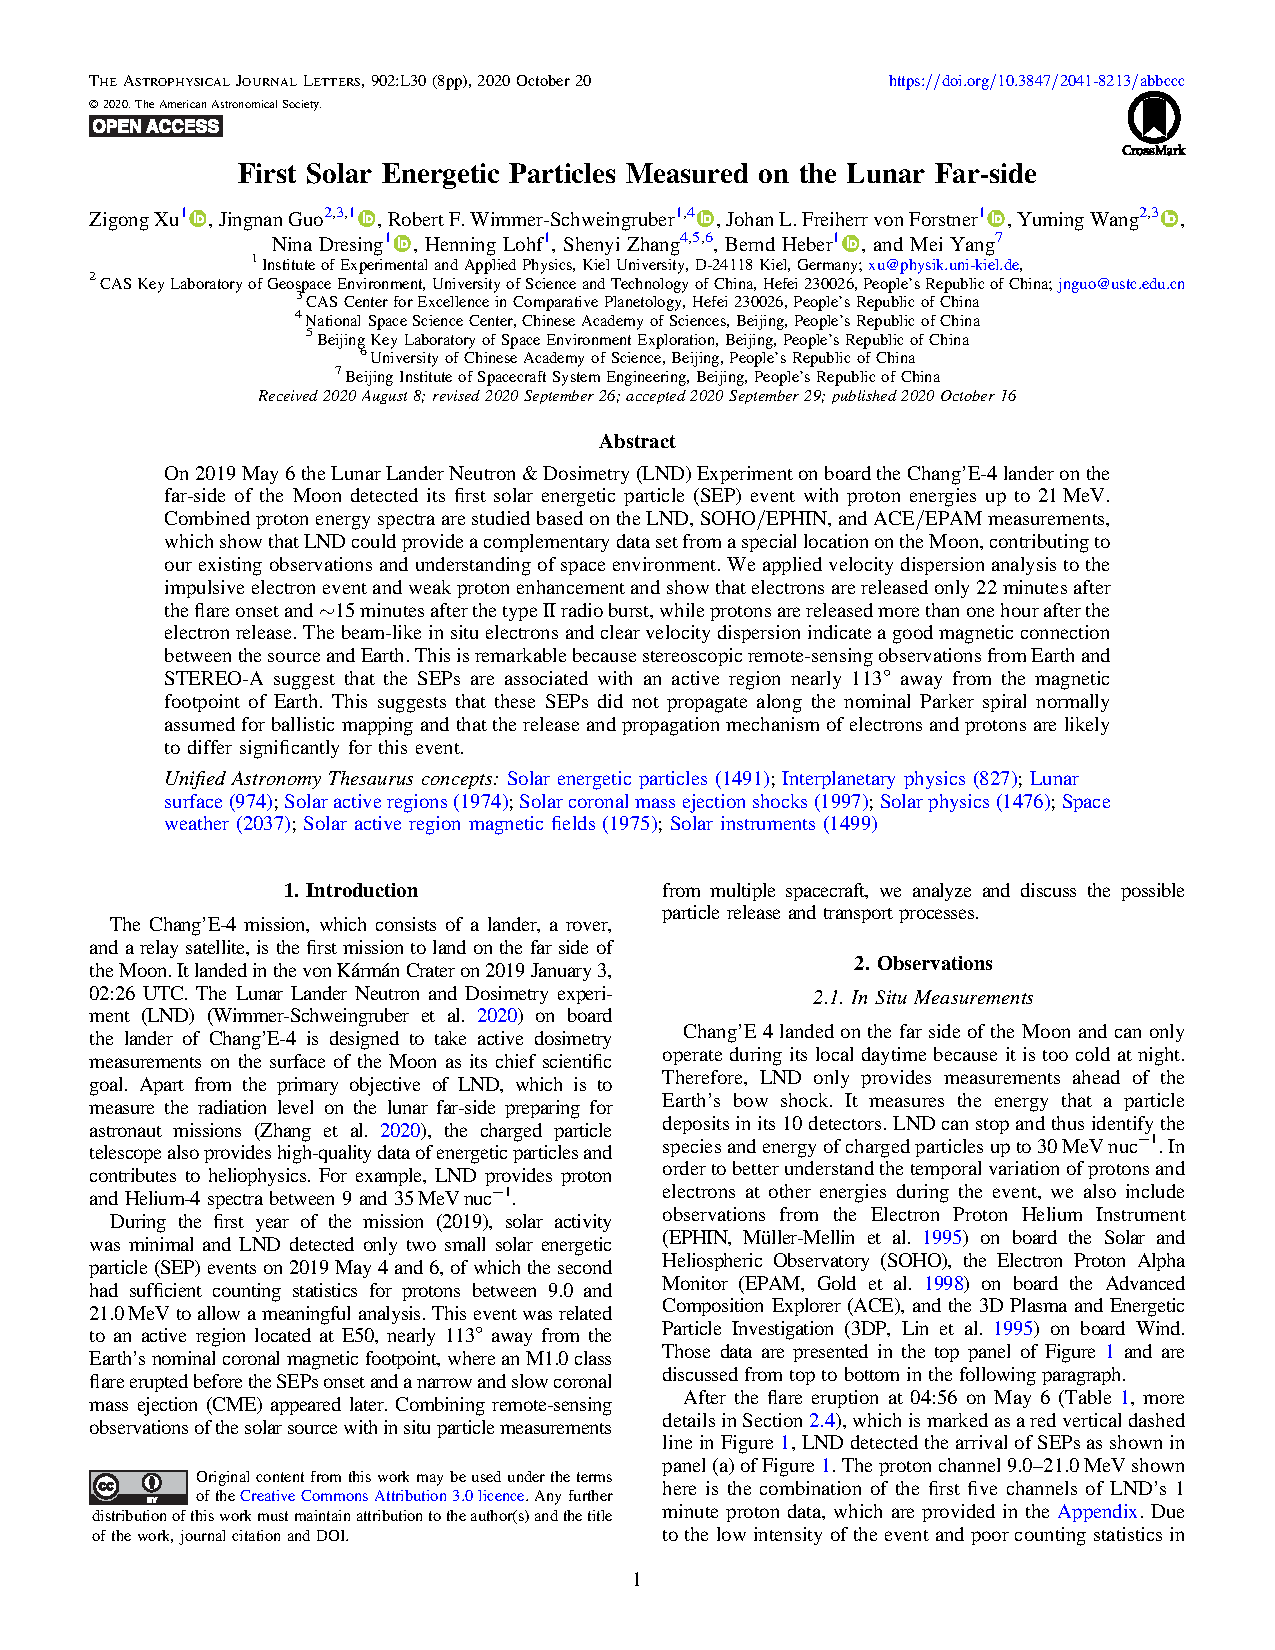
\includepdf[pages={1}, link, linkname=paper_xu2020, scale=.9, pagecommand={\refstepcounter{includepdfpageAPJLTwenty}\label{paper_xu2020.\theincludepdfpageAPJLTwenty}}]{publications/Xu_et_al_2020_ApJL.pdf}
%
\addtocounter{section}{1} 
\phantomsection
\addcontentsline{toc}{section}{\arabic{chapter}.\arabic{section} Observations}
\includepdf[pages={2-4}, link, linkname=paper_xu2020, scale=.9, pagecommand={\refstepcounter{includepdfpageAPJLTwenty}\label{paper_xu2020.\theincludepdfpageAPJLTwenty}}]{publications/Xu_et_al_2020_ApJL.pdf}
%
\addtocounter{section}{1} 
\phantomsection
\addcontentsline{toc}{section}{\arabic{chapter}.\arabic{section} Summary and Discussion}
\includepdf[pages={5-6}, link, linkname=paper_xu2020, scale=.9, pagecommand={\refstepcounter{includepdfpageAPJLTwenty}\label{paper_xu2020.\theincludepdfpageAPJLTwenty}}]{publications/Xu_et_al_2020_ApJL.pdf}
%
\addtocounter{section}{1} 
\phantomsection
\addcontentsline{toc}{section}{\arabic{chapter}.\arabic{section} Appendix}
\includepdf[pages={7}, link, linkname=paper_xu2020, scale=.9, pagecommand={\refstepcounter{includepdfpageAPJLTwenty}\label{paper_xu2020.\theincludepdfpageAPJLTwenty}}]{publications/Xu_et_al_2020_ApJL.pdf}
%
\addtocounter{section}{1} 
\phantomsection
\addcontentsline{toc}{section}{\arabic{chapter}.\arabic{section} References}
\includepdf[pages={8}, link, linkname=paper_xu2020, scale=.9, pagecommand={\refstepcounter{includepdfpageAPJLTwenty}\label{paper_xu2020.\theincludepdfpageAPJLTwenty}}]{publications/Xu_et_al_2020_ApJL.pdf}
